\chapter{Toric Hyperk{\"a}hler Manifolds}

The goal of the first half of this chapter is to introduce the quaternionic analogue to toric symplectic manifolds, which are aptly called \emph{toric hyperk{\"a}hler manifolds}, which were first introduced in \cite{BD00}. In fact, they introduced the more general hypertoric \emph{varieties}, which also included the case of non-smooth spaces, or orbifolds. For brevity, we shall not concern ourselves with the non-smooth cases however. Our notation will follow more closely to that in \cite{Pro04}, which specialises to types of hypertoric manifolds which are essentially analogues to the toric symplectic manifolds we considered in Chapter 2.

\section{Hyperk{\"a}hler Reduction and Hyperk{\"a}hler Analogues}

\subsection{Introduction and Definitions}

A \emph{\HK manifold} is a Riemannian manifold $(M,g)$ equipped with three orthogonal, parallel complex structures $J_{1}, J_{2}, J_{3}$, satisfying the usual quaternion relations. These three complex structures give rise to three symplectic forms
$$
	\w_{1}(v,w) = g(J_{1}v,w),\quad \w_{2}(v,w) = (J_{2}v,w),\quad \w_{3}(v,w) = g(J_{3}v,w),
$$
so that each $(g,J_{i},w_{i})$ is in its own right a \K structure on $M$ for $i = 1,2,3$. The complex-valued two-form $\w_{2} + \sqrt{-1}\w_{3}$ is a closed, non-degenerate, and holomorphic two-form with respect to the complex structure $J_{1}$. Thus any \HK manifold can be considered as a \emph{holomorphic symplectic} manifold with complex structure $J_{1}$, real symplectic form $\w_{\RR} := \w_{1}$, and holomorphic symplectic form $\w_{\CC} := \w_{2} + \sqrt{-1}\w_{3}$.

An action of a Lie group $G$ on a \HK manifold $M$ is called \emph{hyperhamiltonian} if it is hamiltonian with respect to $\w_{\RR}$, and holomorphic hamiltonian with respect to $\w_{\CC}$, with a $G$-equivariant moment map
$$
	\mu_{HK} := \mu_{\RR} \oplus \mu_{\CC} \longrightarrow \mf{g}^{\ast} \oplus \mf{g}_{\CC}^{\ast}.
$$
The following theorem describes the \emph{\HK quotient} construction, which is the quaternionic analogue of a \K quotient:

\begin{thm}[\cite{HKLR87}]
	Let $M$ be a \HK manifold equipped with a hyperhamiltonian action of a compact Lie group $G$, with moment maps $\mu_{1}, \mu_{2}, \mu_{3}$. Suppose that $\xi = \xi_{\RR} \oplus \xi_{\CC}$ is a central regular value for $\mu_{HK}$, and that $G$ acts freely on $\mu_{HK}^{-1}(\xi)/G$. Then there is a unique \HK structure on the \HK quotient $\mf{M} = M\sssslash_{\xi}G := \mu_{HK}^{-1}(\xi)/G$, with associated symplectic and holomorphic symplectic forms $\w_{\RR}^{\xi}$ and $\w_{\CC}^{\xi}$, such that $\w_{\RR}^{\xi}$ and $\w_{\CC}^{\xi}$ pull-back to the restrictions of $\w_{\RR}$ and $\w_{\CC}$ on $\mu_{HK}^{-1}(\xi)$.
\end{thm}
In general, the action of $G$ on $\mu_{HK}^{-1}(\xi)$ will not be free, but only locally free. In this situation, we would end up with a \emph{\HK orbifold}. However in the sequel, we shall only concern ourselves when the action is free, and that $\mf{M}$ is smooth, \ie a manifold.

Let us specialise to the case when $M = T^{\ast}\CC^{n}$, and let $G$ act on $T^{\ast}\CC^{n}$ with the induced action from a linear action of $G$ on $\CC^{n}$, with moment map $\mu : \CC^{n} \rightarrow \mf{g}^{\ast}$. We can identify $\HH^{n}$ with $T^{\ast}\CC^{n}$ such that the complex structure $J_{1}$ on $\HH^{n}$ is given by right multiplication by $i$, and that $J_{1}$ corresponds to the natural complex structure on $T^{\ast}\CC^{n}$. With this identification in mind, $T^{\ast}\CC^{n}$ inherits a \HK structure. The real symplectic form $\w_{\RR}$ is obtained from the sum of the pull-backs of the standard \K forms on $\CC^{n}$ and $(\CC^{n})^{\ast}$, and the holomorphic symplectic form $\w_{\CC}$ is $\w_{\CC} = d\eta$, where $\eta$ is the canonical holomorphic one-form on $T^{\ast}\CC^{n}$.

As $G$ acts $\HH^{n}$-linearly on $T^{\ast}\CC^{n} \cong \HH^{n}$ from the left, the action is hyperhamiltonian with moment map $\mu_{HK} = \mu_{\RR} \oplus \mu_{\CC}$, where
$$
	\mu_{\RR}(z,w) = \mu(z) - \mu(w),\qquad \text{and} \qquad \mu_{\CC}(z,w)(\hat{v}_{z}),
$$
where $w\in T_{z}^{\ast}\CC^{n}$, $v \in \mf{g}_{\CC}$, and $\hat{v}_{z}$ is the vector field in $T_{z}\CC^{n}$ induced by $v$. For a central element $\alpha \in \mf{g}^{\ast}$, we call the specialised \HK quotient
$$
	\mf{M} = T^{\ast}\CC^{n}\sssslash_{(\alpha,0)}G := \big( \mu_{\RR}^{-1}(\alpha) \cap \mu_{\CC}^{-1}(0)\big)/G
$$
the \HK analogue of the corresponding \K quotient,
$$
	\mf{X} = \CC^{n} \sslash_{\alpha} G = \mu^{-1}(\alpha)/G.
$$

We quote the following propositions without proof:

\begin{prop}
	Suppose that $\alpha$ and $(\alpha,0)$ are regular values for $\mu$ and $\mu_{HK}$, respectively. Then the cotangent bundle $T^{\ast}\mf{X}$ is isomorphic to an open subset of $\mf{M}$, and is dense if it is non-empty.
\end{prop}

\subsection{The $\CC^{\ast}$-Action and the Core of a Hyperk{\"a}hler Analogue}

Consider the action of $\CC^{\ast}$ on $T^{\ast}\CC^{n}$ given by
$$
	\hbar \cdot (z,w) = (z,\hbar w),
$$
\ie by scalar multiplication of the cotangent fibre. The holomorphic moment map $\mu_{\CC}:T^{\ast}\CC^{n} \rightarrow \mf{g}_{\CC}^{\ast}$ is $\CC^{\ast}$-equivariant with respect to the scalar action on $\mf{g}_{\CC}^{\ast}$, and hence the $\CC^{\ast}$-action descends to $\mu_{\CC}^{-1}(0)$. Further, this $\CC^{\ast}$-action commutes with the linear action of $G$ on $\CC^{n}$, and consequently the action of $\CC^{\ast}$ is $J_{1}$-holomorphic on $\mf{M} = \big(\mu_{\RR}^{-1}(\alpha) \cap \mu_{\CC}^{-1}(0)\big)/G$. However, the $\CC^{\ast}$-action \emph{does not} preserve the holomorphic symplectic form nor the \HK structure on $\mf{M}$; rather it scales $\m_{\CC}$ with ``homogeneity one'', \ie $\hbar^{\ast}\w_{\CC} = \hbar \w_{\CC}$ for any $\hbar\in \CC^{\ast}$.

Given that $\mf{M}$ is smooth, the action of the compact subgroup $S^{1} \subset \CC^{\ast}$ is hamiltonian with respect to the real symplectic two-form $\w_{\RR}$, with corresponding moment map $\Phi[z,w] = \tfrac{1}{2}\|w\|^{2}$. This map is a perfect Morse-Bott function, and its image is contained in $\RR_{\geq 0}$. Further, we note that $\Phi^{-1}(0) = \mf{X} \subset \mf{M}$. The following proposition will be instrumental in the sequel, though again we quote it without proof:

\begin{prop}
	If the original moment map for the $G$-action on $\CC^{n}$, $\mu: \CC^{n} \rightarrow \mf{g}^{\ast}$, if proper, then so is the moment map for the $S^{1}$ action, $\Phi:\mf{M} \rightarrow \RR_{\geq 0}$.
\end{prop}

Next we shall define what is known as the \emph{core} of a \HK analogue, which will be essential in describing the fixed points of the $\CC^{\ast}$-action of $\mf{M}$.

\begin{defn}
	Suppose that $\mf{M}$ is smooth and $\Phi$ is proper. The \emph{core} $\mc{L} \subset \mf{M}$ of the hypertoric variety is defined to be the union of the $\CC^{\ast}$ orbits whose closures are compact.
\end{defn}

Let $F$ be a connected component of $\mf{M}^{S^{1}} =  \mf{M}^{\CC^{\ast}}$, and let $U_{F}$ be the closure of the set of points $p \in \mf{M}$ such that $\lim\limits_{\hbar \rightarrow \infty} \hbar \cdot p \in F$.

\begin{prop}[\cite{proudfoot2004hyperkahler}; Proposition 2.8]
	The core $\mc{L} \subset \mf{M}$ has the following properties:
	\begin{enumerate}
		\item $\mc{L}$ is an $S^{1}$-equivariant deformation retract of $M$;
		\item $U_{F}$ is isotropic with respect to the holomorphic symplectic form $\w_{\CC}$;
		\item Provided that $\mf{M}$ is smooth at $F$, then $\dim U_{F} = \tfrac{1}{2}\dim \mf{M}$.
	\end{enumerate}
\end{prop}

\section{Hypertoric Manifolds}

\subsection{Definition}

In this section, we shall specialise further now to when a \HK analogue $\mf{M}$ is the analogue to a toric symplectic manifold $\mf{X} = \mu^{-1}(\alpha)/N$, \ie we replace the compact Lie group $G$ with the torus $N = \ker(\pi:T^{n} \rightarrow T^{d})$, using the same notation as in the second chapter. 

Recall the short exact sequence of tori:
\[
\begin{tikzcd}
1 \arrow[r] & N \arrow[r, hook, "i"] & T^{n} \arrow[r, "\pi"] &
T^{d} \arrow[r] & 1,
\end{tikzcd}
\]
and extend the linear action of the torus $N$ on $\CC^{n}$ to $T^{\ast}\CC^{n}$. This action is trihamiltonian and we obtain the following \HK moment map
$$
	\mu_{HK} = \mu_{\RR} \oplus \mu_{\CC} :T^{\ast}\CC^{n} \longrightarrow \mf{n}^{\ast} \oplus \mf{n}_{\CC}^{\ast},
$$
where
$$
	\mu_{\RR}(z,w) = i^{\ast}\bigg( \frac{1}{2}\sum_{i=1}^{n}( |z_{i}|^{2} - |w_{i}|^{2})\partial_{i} \bigg),\quad \text{and}\quad \mu_{\CC}(z,w) = i_{\CC}^{\ast}\bigg( \sum_{i=1}^{n}(z_{i}w_{i}) \partial_{i} \bigg).
$$
Given an element $\alpha \in \mf{n}^{\ast}$ with a corresponding lift $\lambda = (\lambda_{1},\ldots, \lambda_{n}) \in (\RR^{n})^{\ast}$, the \K quotient
$$
	\mf{X} = \CC^{n}\sslash_{\alpha}N = \mu^{-1}(\alpha)/N
$$
is our usual toric symplectic manifold with residual $T^{d}$-action from before, and moreover its \HK analogue
$$
	\mf{M} = T^{\ast}\CC^{n} \sssslash_{(\alpha,0)} N = \big( \mu_{\RR}^{-1}(\alpha) \cap \mu_{\CC}^{-1}(0)\big)/N
$$
is what we shall call a \emph{hypertoric manifold}\footnote{More generally, $\mf{M}$ should be called a hypertoric variety, and only call $\mf{M}$ a manifold when it is smooth. However, we shall restrict our attention to the smooth case for simplicity.}. The hypertoric manifold $\mf{M}$ also admits a residual action of the torus $T^{d}$, which is hyperhamiltonian with \HK moment map
$$
	\phi_{HK} := \phi_{\RR} \oplus \phi_{\CC}: \mf{M} \longrightarrow (\RR^{d})^{\ast} \oplus (\CC^{d})^{\ast},
$$
where
\begin{equation*}
	\begin{split}
		\prr[z,w] &= \frac{1}{2}\sum_{i=1}^{n}(|z_{i}|^{2} - |w_{i}|^{2} - \lambda_{i})\partial_{i} \in \ker(i^{\ast}) = (\RR^{d})^{\ast},\\
		\pcc[z,w] &= \sum_{i=1}^{n}(z_{i}w_{i}) \partial_{i} \in \ker(i_{\CC}^{\ast}) = (\CC^{d})^{\ast}.
	\end{split}
\end{equation*}

\subsection{Hyperplane Arrangements}

A fundamental difference between the toric manifold $\mf{X}$ and the hypertoric manifold $\mf{M}$ is that the \HK moment map for $\mf{M}$ is surjective, and that $\mf{M}$ is non-compact. Despite this, we can still describe the image of the real moment map $\prr:\mf{M}\rightarrow (\RR^{d})^{\ast}$ combinatorially by means of a \emph{hyperplane arrangement}. To describe this arrangement, recall that the map $\pi:\RR^{n}\rightarrow \RR^{d}$ was defined by $\pi(e_{i}) = u_{i}$, for $i = 1,\ldots, n$, where the $u_{i}$ were the primitive, integral, inward-pointing normal vectors to the hyperplanes that determined our Delzant polytope. In the hypertoric case, they instead now describe a collection of \emph{affine hyperplanes} $H_{i} \subset (\RR^{d})^{\ast}$ as follows: consider
$$
	H_{i} = \{ v \in (\RR^{d})^{\ast}\st v \cdot u_{i} + \lambda_{i} = 0 \},
$$
so that the $u_{i} \in \ZZ^{d}$ is the normal vector to the hyperplane $H_{i}$. The hyperplane $H_{i}$ divides $(\RR^{d})^{\ast}$ into two half-spaces
\begin{equation*}
	\begin{split}
		F_{i} &= \{v \in (\RR^{d})^{\ast}\st v \cdot u_{i} + \lambda_{i} \geq 0\},\\
		G_{i} &= \{v \in (\RR^{d})^{\ast} \st v \cdot u_{i} + \lambda_{i} \leq 0  \}.
	\end{split}
\end{equation*} 
Let
$$
	\Delta = \bigcap_{i=1}^{n}F_{i} = \{v \in (\RR^{d})^{\ast} \st v \cdot u_{i} + \lambda_{i} \geq 0, \text{ for all } i = 1,\ldots, n  \}
$$
be the (possibly empty) polyhedron in $(\RR^{d})^{\ast}$ defined by the affine hyperplane arrangement $\mc{A} = \{H_{1},\ldots, H_{n}  \}$. We note that choosing a different lift $\lambda^{\prime}$ of $\alpha$ corresponds combinatorially to translating the arrangement $\mc{A}$ inside of $(\RR^{d})^{\ast}$, and geometrically to shifting the \K and \HK moment maps for the residual $T^{d}$-action by $\lambda^{\prime} - \lambda \in \ker (i^{\ast}) = (\RR^{d})^{\ast}$.

We shall call that the arrangement $\mc{A}$ \emph{simple} if every subset of $m$ hyperplanes with non-empty intersection intersects with codimension $m$, and call $\mc{A}$ \emph{smooth} if every collection of $d$ linearly-independent vector $\{u_{i_{1}},\ldots, u_{i_{d}}  \}$ spans $(\RR^{d})^{\ast}$. The reason for this terminology is the following proposition.

\begin{prop}
	The hypertoric variety $\mf{M}$ is an orbifold if and only if $\mc{A}$ is simple, and $\mf{M}$ is smooth if and only if $\mc{A}$ is smooth.
\end{prop}

As we wish to restrict our attention to the case where $\mf{M}$ is a manifold, we shall assume in the sequel that $\mc{A}$ is a smooth arrangement of hyperplanes.

\subsection{The Core of a Hypertoric Manifold}

The holomorphic moment map $\pcc:\mf{M} \rightarrow (\CC^{d})^{\ast}$ is $\CC^{\ast}$-equivariant with respect to the scalar action of $\CC^{\ast}$ on $(\CC^{d})^{\ast}$, hence both the core $\mc{L}$ and the fixed-point set $M^{\CC^{\ast}}$ will be contained in
\begin{equation*}
	\mc{E}:= \pcc^{-1}(0) = \bigg\{ [z,w] \in \mf{M} \st z_{i}w_{i} = 0,\ 1 \leq i \leq n \bigg\}.
\end{equation*}

\begin{defn}
	We shall call $\mc{E}$ the \emph{extended core} of $\mf{M}$.
\end{defn}

The restriction of $\prr|_{\mc{E}}: \mc{E} \rightarrow (\RR^{d})^{\ast}$ is surjective from the defining equations, and further the extended core naturally breaks up into components
\begin{equation*}
	\mc{E}_{A} :=  \bigg\{ [z,w] \in \mc{E} \st w_{i} = 0 \text{ for all } i \in A\text{ and } z_{i} = 0 \text{ for all } i \not\in A \bigg\},
\end{equation*}
where $A \subseteq \{1,\ldots, n\}$ is an indexing set. The hyperplanes $\{ H_{i}  \}_{i=1}^{n}$ divide $(\RR^{d})^{\ast}$ into a union of convex polyhedra
\begin{equation*}
	\Delta_{A} = \bigg(\bigcap_{i\in A} F_{i}   \bigg) \cap \bigg( \bigcap_{i\not\in A} G_{i}.   \bigg),
\end{equation*}
some of which may be empty.

\begin{lem}
	If $w_{i} = 0$ then $\im(\prr) \subseteq F_{i}$, and if $z_{i} = 0$ then $\im(\prr) \subseteq G_{i}$.
\end{lem}

\begin{proof}
	Let $y \in (\RR^{d})^{\ast}$ be the image of the moment map $\prr$ for a point $[z,w] \in \mc{E}$, then
	\begin{equation*}
		y \cdot u_{i} + r_{i} = \mrr(z,w) \cdot e_{i} = \frac{1}{2}\Big( |z_{i}|^{2} - |w_{i}|^{2} \Big),
	\end{equation*}
	and hence $y \geq 0$ if $i \in A$, and $y \leq 0$ if $i \not\in A$.
\end{proof}


\begin{figure}[h!]
	%		\centering
	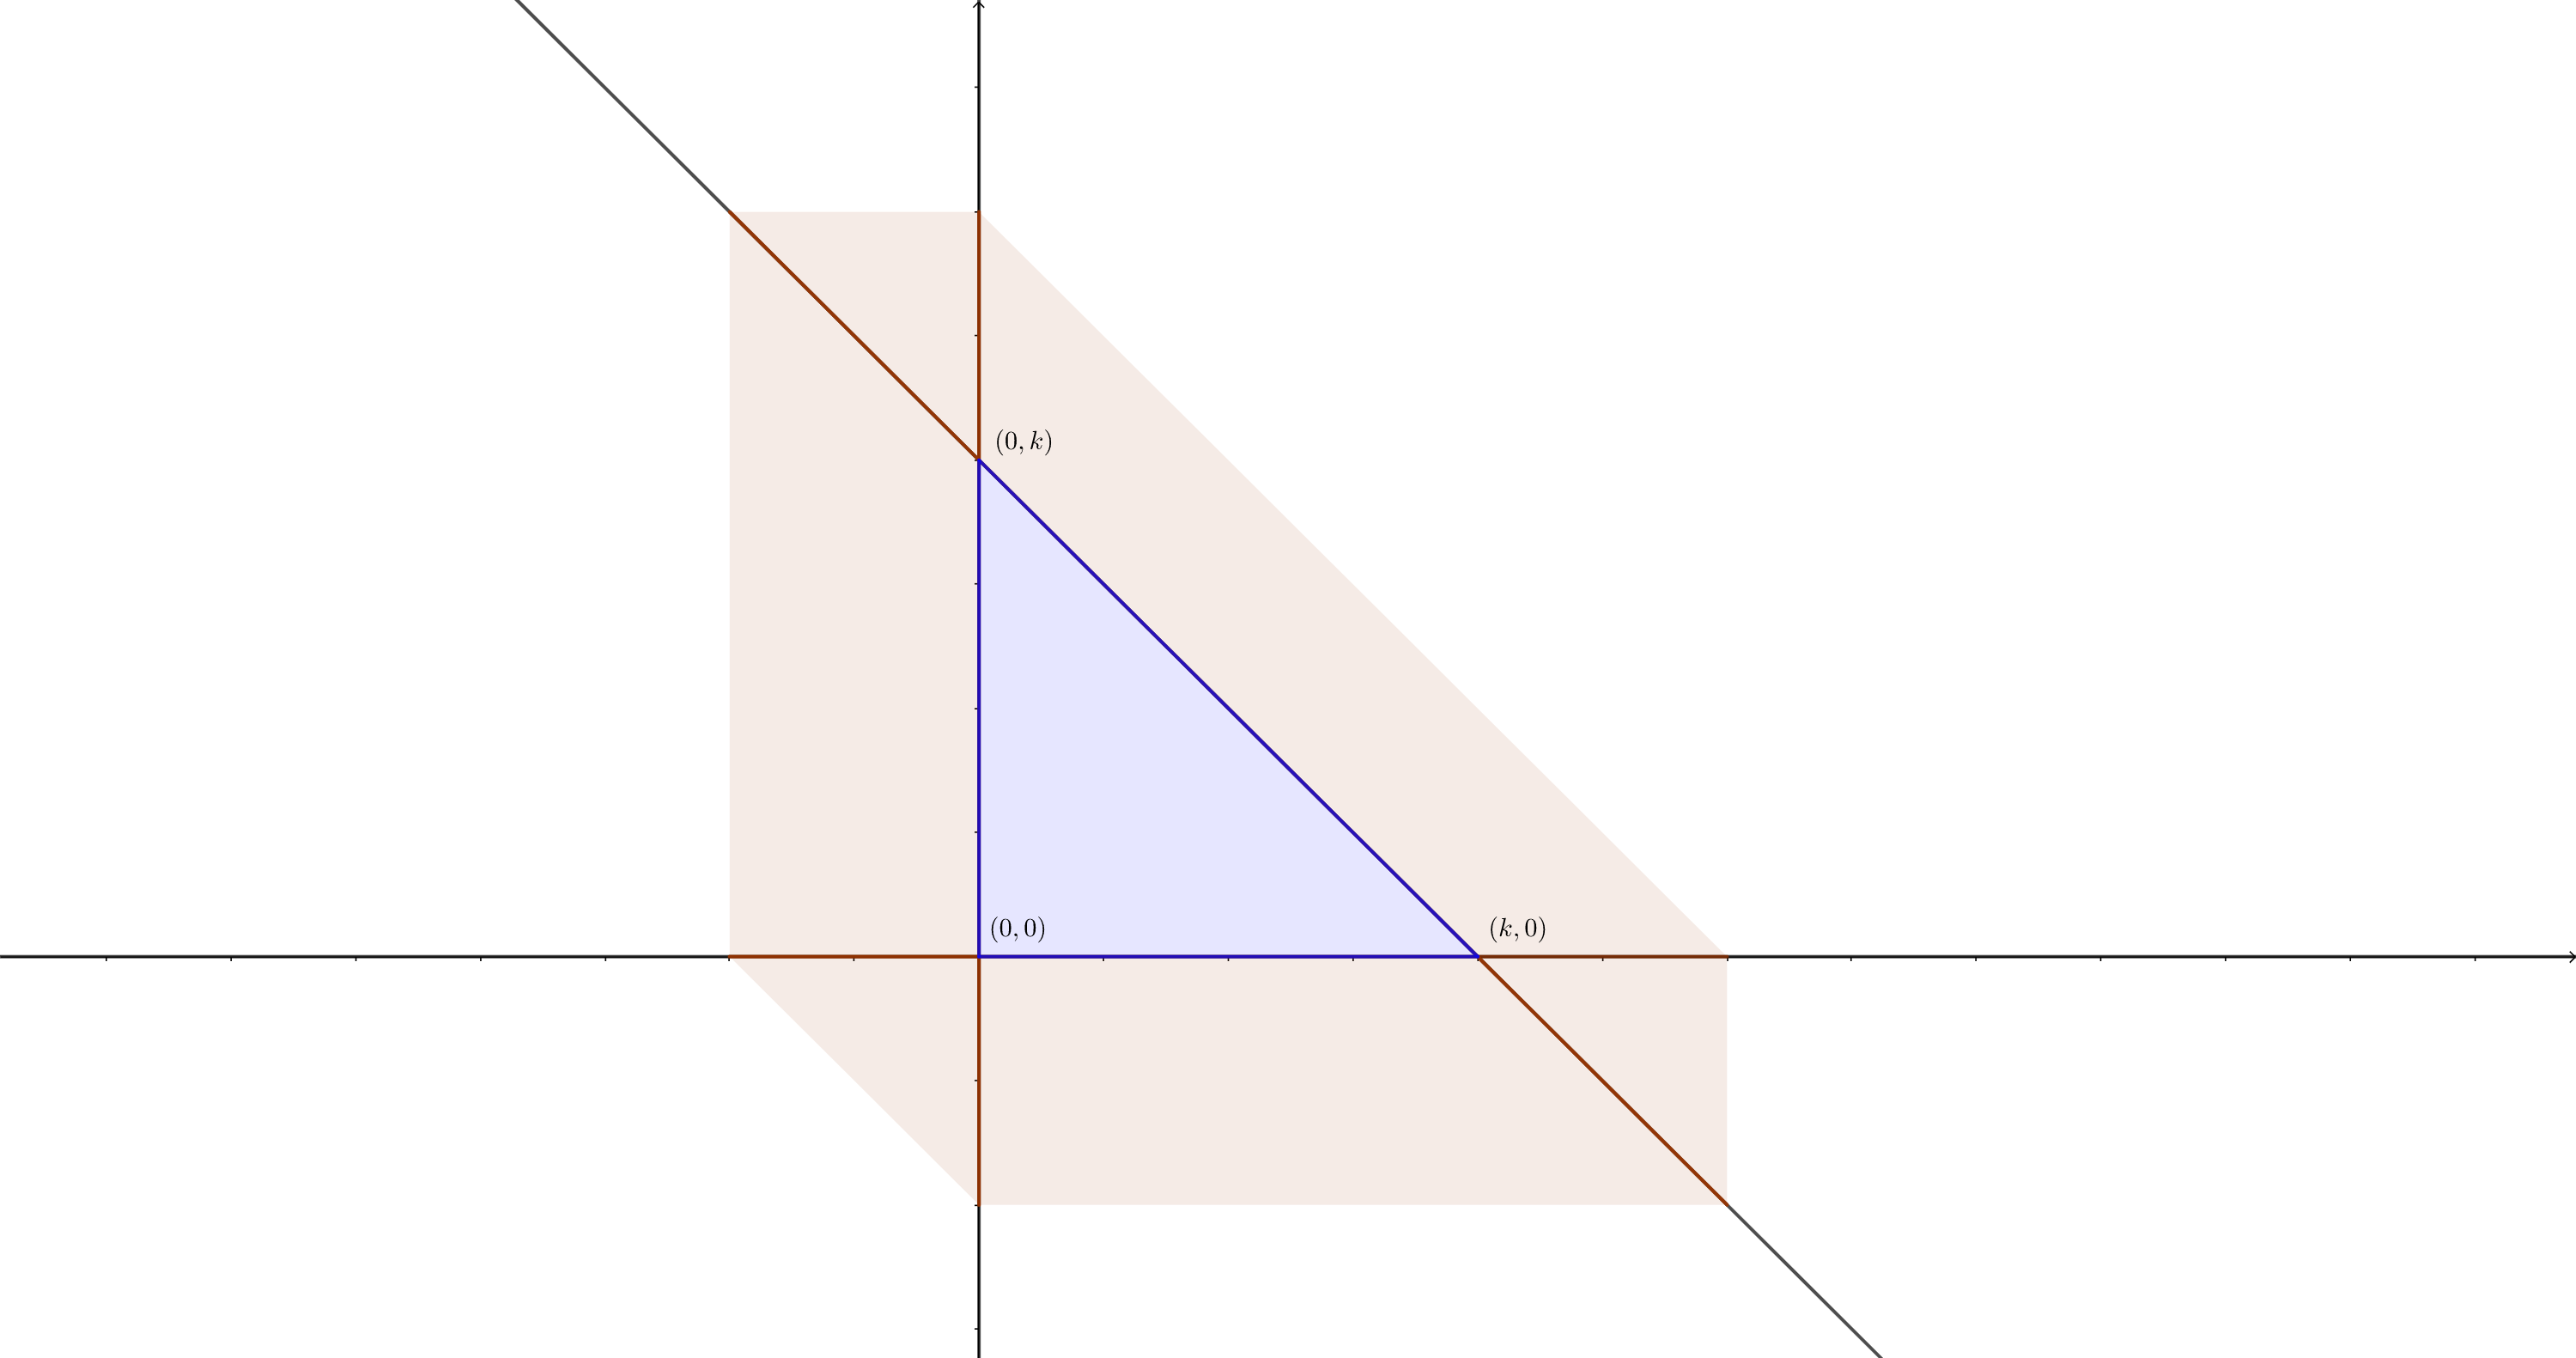
\includegraphics[width=1.2\linewidth]{Cotangent_CP2.png}
	\caption{The image of $\prr(M)$ for $\mf{M} \cong T^{\ast}\CC\PP^{2}$.}
	\label{fig:test1}
\end{figure}

\begin{lem}
	The component $\mc{E}_{A}$ of the extended core is isomorphic to the toric variety corresponding to the polytope $\Delta_{A}$.
\end{lem}

The $\CC^{\ast}$-action does not act as a sub-torus of $T_{\CC}^{d}$ on $M$ globally, but when restricted to each component $\mc{E}_{A}$ of the extended core it does in a combinatorial fashion that we shall now describe.

Consider a component $\mc{E}_{A} \subset \mc{E}$, then for some $[z,w] \in \mc{E}_{A}$ and $\hbar \in \CC^{\ast}$:
\begin{equation*}
	\hbar \cdot [z,w] = [z,\hbar w] = [\hbar_{1} z_{1}, \ldots, \hbar_{n} z_{n}, w_{1}, \ldots , w_{n}     ],\qquad \text{where } \hbar_{i} = 
	\begin{cases}
	\hbar^{-1}\qquad &\text{if } i \in A,\\
	1\qquad &\text{if } i \not\in A.
	\end{cases}
\end{equation*}
This shows that the restriction of the $\CC^{\ast}$-action to the component $\mc{E}_{A}$ is the one-dimensional sub-torus $(\CC^{\ast})_{A} := (\hbar_{1}, \ldots, \hbar_{n})$ of the original torus $T_{\CC}^{n}$, which we can then restrict to the circle subgroup $S_{A} \subset T^{n}$.

For $B \subseteq \{1,\ldots, n\}$, denote by $\mc{E}_{A}^{B}$ the subvariety of the extended core component $\mc{E}_{A}$ defined by
\begin{equation*}
	\mc{E}_{A}^{B} := \mc{E}_{A} \cap \{z_{j} = 0 = w_{j}\}
\end{equation*}
which may be empty. In $(\RR^{d})^{\ast}$, this corresponds to the intersection of the polyhedron $\Delta_{A}$ with the collection of hyperplanes $\{ H_{j}  \}_{j \in B}$, that is
\begin{equation*}
	\Delta_{A}^{B} = \bigg( \bigcap_{j \in B} H_{j} \bigg) \cap \Delta_{A}.
\end{equation*}

\begin{prop}
	The fixed point set of the $S^{1}$-action on $\mc{E}_{A}$ is the union of those toric subvarieties $\mc{E}_{A}^{B}$ such that $\sum_{i\in A} u_{i}$ lies in $\text{Span}_{j \in B} u_{j}$.
\end{prop}

\begin{cor}
	Every vertex $v \in (\RR^{d})^{\ast}$ of the polyhedral complex given by our arrangement is the image of an $S^{1}$-fixed point in $\mf{M}$. Every component of $\mf{M}^{S^{1}}$ maps to a face of the polyhedral complex.
\end{cor}

\section{Compactifying the Hypertoric Variety via Symplectic Cutting}

In the sequel, we shall want to try and associate to $\mf{M}$ a ``canonical Hilbert space'' $\mc{Q}(\mf{M})$, which will consist of a subspace of the space of global holomorphic sections to some ``prequantum'' line bundle, by means of the geometric quantisation construction which we shall discuss later. As $\mf{M}$ is non-compact, the space $\mc{Q}(\mf{M})$ will be infinite-dimensional. However, because of the $\CC^{\ast}$-action, we can instead consider the weight spaces in $\mc{Q}(\mf{M})$ of the $S^{1} \subset \CC^{\ast}$-action, which will have a compact fixed point loci. Hence the individual weight spaces will be finite dimensional, and a lot more tractable to work with. For this consideration, we can compactify $\mf{M}$ by Lerman's symplectic cutting technique \cite, since the moment map for the $S^{1}$-action, $\Phi:\mf{M} \rightarrow \RR_{\geq 0}$ is proper. The contents of this section is original work, though a similar construction is done in \cite{Hau98} to compactify Higgs bundle moduli\footnote{In fact, in section 4 of \cite{Hau98}, it is stated that it would be an interesting task to apply the same idea to the toric \HK varieties of \cite{BD00}.}.

\subsection{General Set-Up}

We will use the $S^{1}$-action to symplectically cut the toric \HK manifold $\mf{M}$ in order to compactify it as follows: consider the product $\mf{M} \times \CC$, where now $S^{1}$ acts on $\mf{M} \times \CC$ as
$$
e^{i\theta} \cdot \big( [z,w], \xi   \big) = \big( [z,e^{i\theta}], e^{i\theta}\xi\big),
$$
which is hamiltonian with moment map
\begin{equation*}
\begin{split}
\mu_{\text{cut}}: \mf{M} \times \CC &\longrightarrow \RR_{\geq 0}, \\
\mu_{\text{cut}}\big( [z,w], \xi  \big) &= \Phi[z,w] + \tfrac{1}{2}|\xi|^{2} - \e,
\end{split}
\end{equation*}
for some $\e \in \RR_{\geq 0}$. Then we have
\begin{equation*}
\begin{split}
\mu_{\text{cut}}^{-1}(0) &= \big\{ ([z,w],\xi) \in M \times \CC \st \|w\|^{2} + |\xi|^{2} = 2\e    \big\} \\
&= \big\{ [z,w] \in M \st \|w\|^{2} = 2\e    \big\} \bigsqcup \big\{ ([z,w],\xi) \in M \times \CC \st |\xi| = \pm\sqrt{2\e - \|w\|^{2}} \big\} \\
&= \big\{ [z,w] \in M \st \|w\|^{2} = 2\e    \big\} \bigsqcup \big\{ ([z,w],\xi) \in M \times \CC \st \xi = e^{i\arg(\xi)}\sqrt{2\e - \|w\|^{2}}    \big\} \\
&= \Phi^{-1}(\e) \bigsqcup (\mf{M} \times S^{1}) \\
&=: \Sigma_{1} \bigsqcup \Sigma_{2},
\end{split}
\end{equation*}
where $\Sigma_{1}$ is just the level-set of $\Phi$ at the level $\e$ in $\mf{M}$, and $\Sigma_{2} = \mf{M} \times S^{1}$ is exhibited as a trivial $S^{1}$-bundle over $\Sigma_{2}$, using the globally defined section
\begin{equation*}
	\mf{M} \rightarrow \mf{M} \times S^{1}, \qquad [z,w] \longmapsto \big( [z,w], e^{i\theta}\sqrt{2\e - \|w\|^{2}}\big), \qquad e^{i\theta} \in S^{1}.
\end{equation*}
Finally, taking the quotient of $\m_{\text{cut}}^{-1}(0)$ by the $S^{1}$-action, we obtain the symplectic cut
\begin{equation*}
	M_{\leq \e} := \m_{\text{cut}}^{-1}(0)/S^{1} = \Sigma_{1}/S^{1} \bigsqcup \Sigma_{2}/S^{1},
\end{equation*}
where $\Sigma_{1}/S^{1} = \Phi^{-1}(\e)/S^{1}$ is just the symplectic reduction, and where $\Sigma_{2}/S^{1}$ is diffeomorphic to $M$ for $\|w\|^{2} < 2\e$, which we denote by $\mf{M}_{<\epsilon}$.

\subsection{Restriction to an Extended Core Component, $\mc{E}_{A}$}

Since the residual circle $S^{1}$-action acts as a subgroup of the original torus $T^{n}$ when restricted to each component $\mc{E}_{A}$ of the extended core $\mc{E}$, we can described combinatorially the resulting configuration of the hyperplane arrangement in $(\RR^{d})^{\ast}$ from taking the cut. For each component, let $j_{A}: \mf{s}^{1} \rightarrow \RR^{n}$ be the derivative of the inclusion of $S^{1}$ into $T^{n}$ on the Lie algebra level, that is
\begin{equation*}
	j_{A}( \xi  ) = (\xi_{1},\ldots, \xi_{n}),\qquad \text{where } \xi_{i} = 
	\begin{cases}
	-1\qquad&\text{if } i\in A,\\
	0\qquad &\text{if } i \not\in A,
	\end{cases}
\end{equation*}
so that its image in $\RR^{n}$ generates a circle subgroup $S^{1}$ in $T^{n}$ that depends on each component $\mc{E}_{A}$. Then the moment map for this restriction for the $S^{1}$-action is
\begin{equation*}
	\Phi[z,w] = j_{A}^{\ast} \circ \mrr[z,w] = \bigg\langle \mrr(z,w), \sum_{i\in A}\xi_{i} u_{i} \bigg\rangle,
\end{equation*}
and so from our above discussion of how we constructed the symplectic cut, the image in $(\RR^{d})^{\ast}$ of the symplectic quotient $\Phi^{-1}(\e)/S^{1}$ is
\begin{equation*}
	\prr(\Phi^{-1}(\e)) = \bigg\{ y \in \Delta_{A} \st \bigg\langle y, \sum_{i\in A}\xi_{i}u_{i}\bigg\rangle + \e = 0 \bigg\} =: H_{A}
\end{equation*}
which introduces an inward-pointing half-space
\begin{equation*}
	F_{A} := \bigg\{ y \in \Delta_{A} \st \bigg\langle y, \sum_{i\in A}\hbar_{i}u_{i}\bigg\rangle + \e \geq 0 \bigg\}
\end{equation*}
such that the image of the extended core component $\mc{E}_{A}$ after being compactified is the original convex polytope $\Delta_{A}$ intersected with $H_{A}$. One can also see clearly that the symplectic quotient $\Phi^{-1}(\e)/S^{1}$ has the restricted $S^{1}$-action as its stabiliser subgroup since, by definition of $H_{A}$, the moment map $\Phi|_{\mc{E}_{A}}$ equals the hyperplane $H_{A}$, \ie $\Phi|_{\mc{E}_{A}}$ is constant along $\Phi^{-1}(\epsilon)/S^{1}$.

\begin{rmk}
	If we had used instead the following action for $S^{1}$
	\begin{equation*}
		e^{i\theta}\cdot \big( [z,w], \xi \big) = \big( [z,e^{i\theta}w], e^{-i\theta}\xi \big)
	\end{equation*}
	with respective moment map
	\begin{equation*}
		\m_{\text{cut}} ([z,w],\xi) = \frac{1}{2}\|w\|^{2} - \frac{1}{2}|\xi|^{2} - \e,
	\end{equation*}
	and taken the cut, then the resulting then we would obtain the other ``discarded half'' $\mf{M}_{>\e}$ of the hypertoric manifold $\mf{M}$ along with the symplectic quotient $\Phi^{-1}(\e)/S^{1}$ with the opposite orientation:
	\begin{equation*}
		\mf{M}_{\geq \e} = \mf{M}_{> \e} \bigsqcup \Big(-(\Phi^{-1}(\e)/S^{1})\Big).
	\end{equation*}
	The component $M_{\e}$ is non-compact however, so we focus on $M_{<\e}$.
\end{rmk}

The following two figures show the resulting moment polytope after compactification, for the hypertoric varieties $T^{\ast}\CC\PP^{2}$ and $T^{\ast}\CC\PP^{3}$. For an interactive figure for the latter, go to: \href{https://www.geogebra.org/classic/suqdctbh}{https://www.geogebra.org/classic/suqdctbh}.

\begin{figure}[h!]
%		\centering
		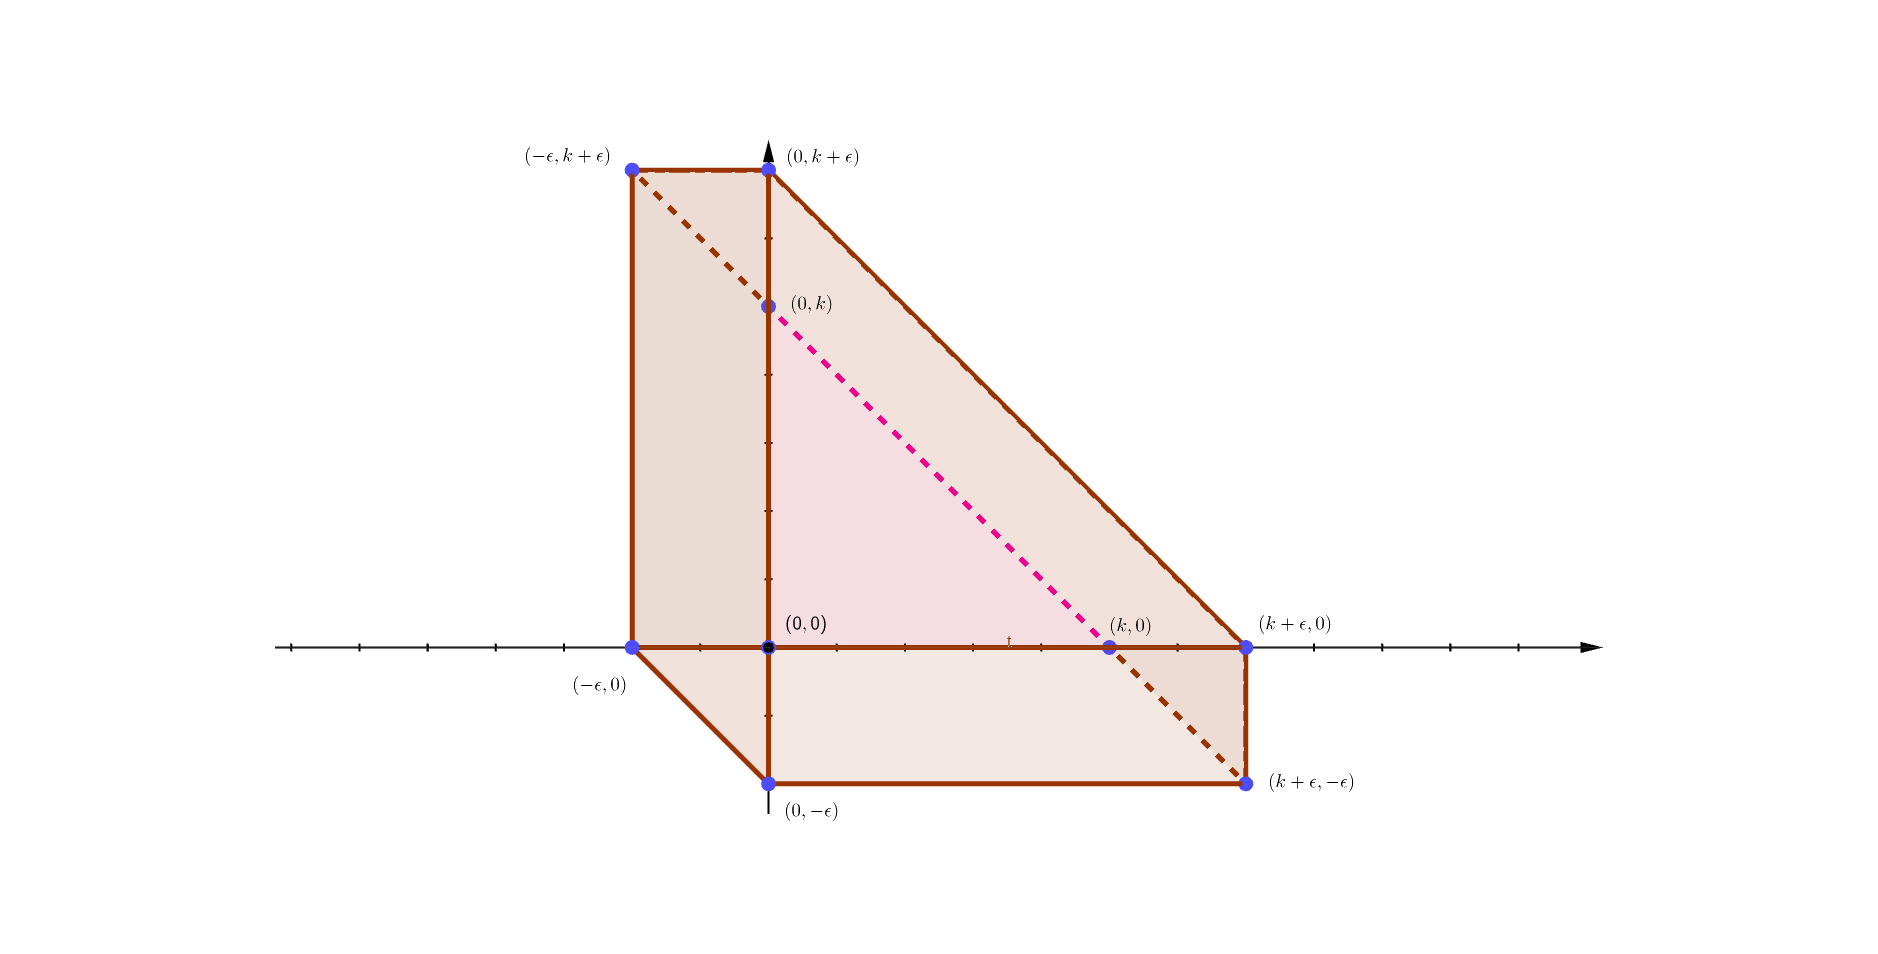
\includegraphics[width=1.2\linewidth]{Symplectic_Cut_Cotangent_CP2.png}
		\caption{The image of $\prr$ for $T^{\ast}\CC\PP^{2}$ after cutting.}
		\label{fig:test1}
\end{figure}

\begin{figure}[h!]
%	\centering
	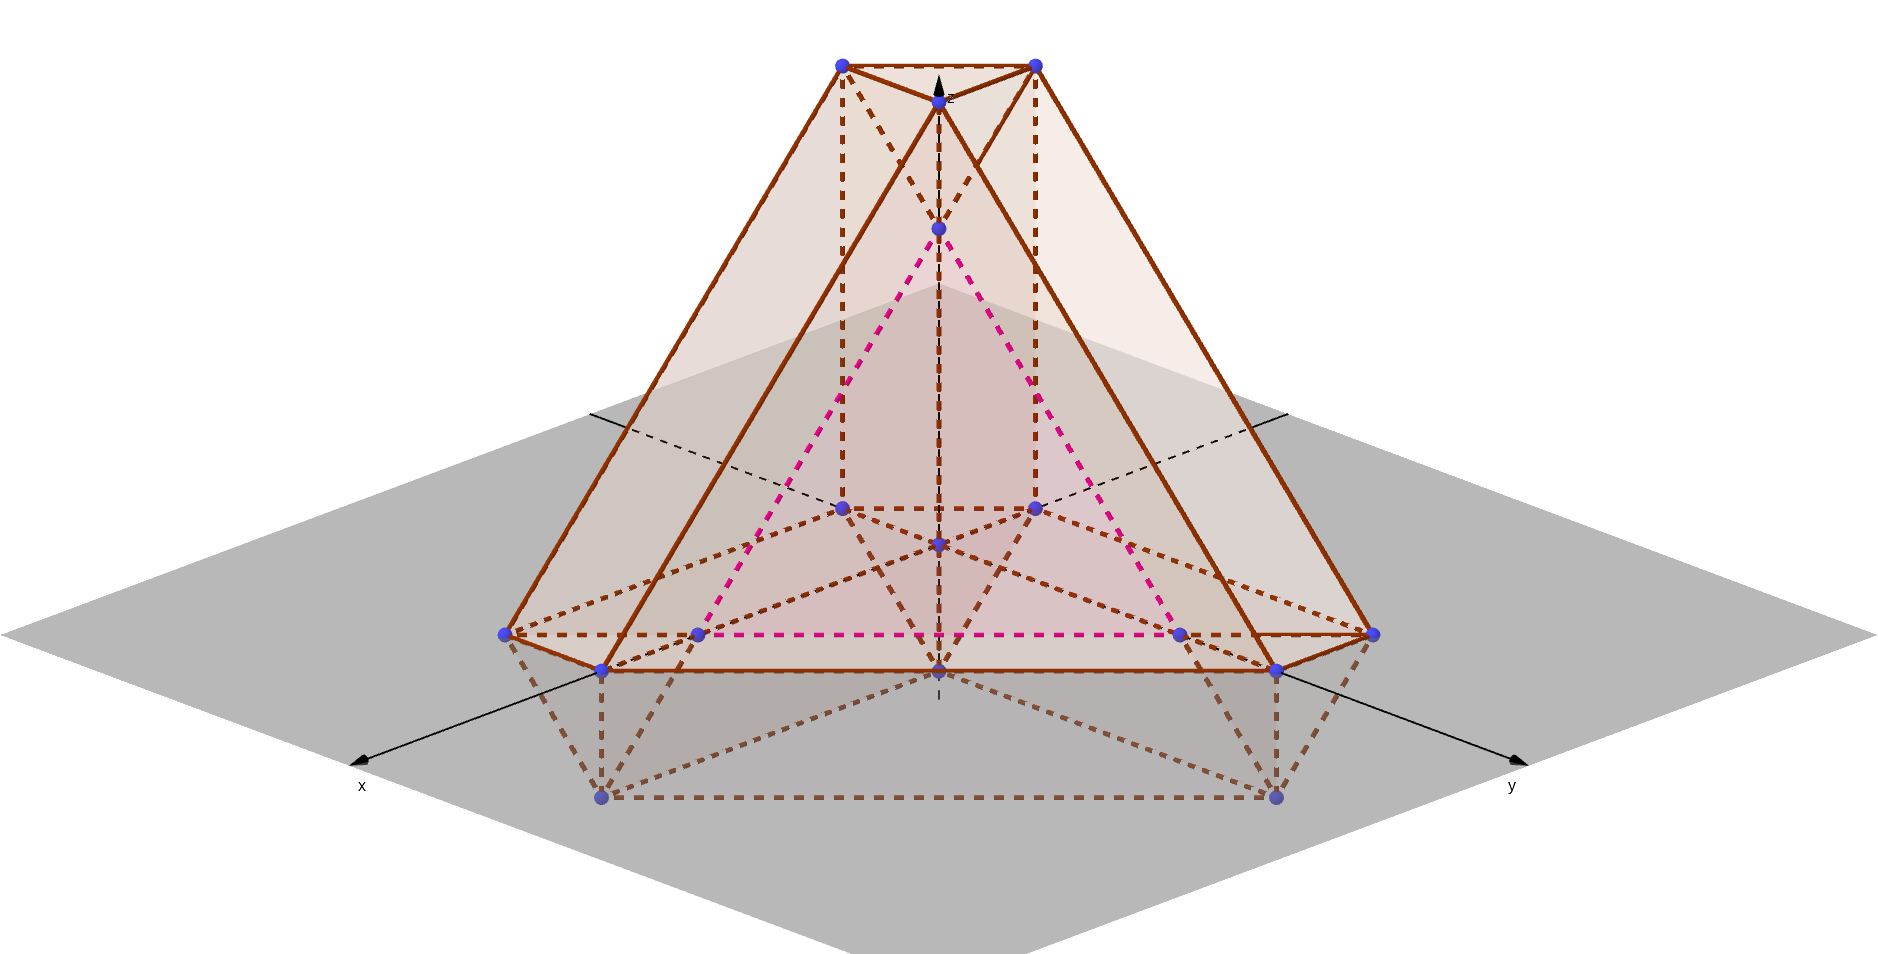
\includegraphics[width=1\linewidth]{Symplectic_Cut_Cotangent_CP3.png}
	\caption{The image of $\prr$ for $T^{\ast}\CC\PP^{3}$ after cutting.}
	\label{fig:test1}
\end{figure}


